\chapter{实验测试技术}
\section{Digital Image Correlation Measurements(DIC)}
DIC技术自从上个世纪八十年代被发明\cite{Sutton1983Determination}以来,作为一种非接触的基于数字灰度图像的全视野的图像分析方法,在确立物体的轮廓和位移方面得到了广泛的应用。\\
\begin{figure}
\centering   
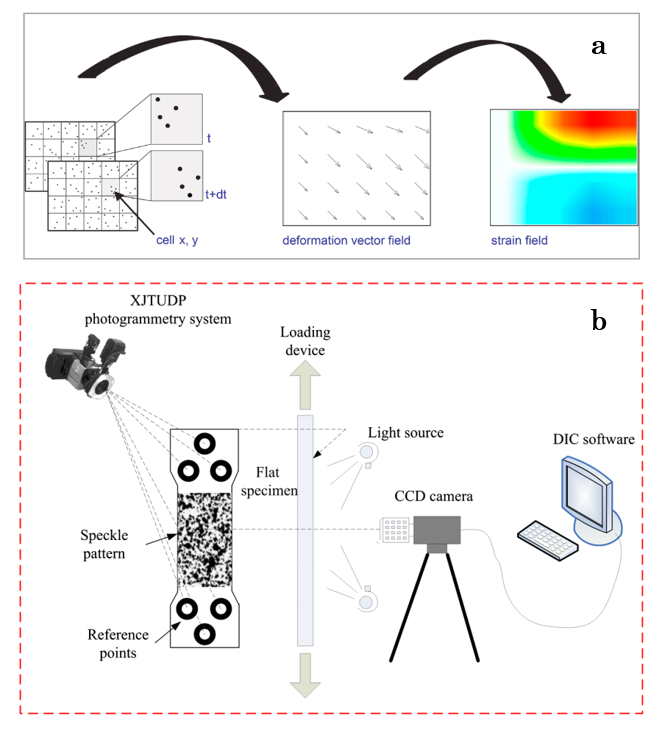
\includegraphics[width=0.8\textwidth]{DIC.png}
\caption{(a)DIC测量位移原理图(b)2D-DIC装置图\cite{Tang2012Photogrammetry}}
\label{fig:dic}
\end{figure}
\indent 如图\ref{fig:dic}(a)所示,DIC可以得到整个测试表面的位移和应变。其依据的原理是通过输入不同时刻的散斑图像进行比对,可以准确地得到全场的位移和应变输出(装置和流程图见图\ref{fig:dic}(b))。由于其全场同时测量和非接触测量的特性,DIC技术在包括实验力学在内的多个学科中发挥了重要作用。
\section{Energy Dispersive Spectrdmeter}
\begin{figure}
\centering   
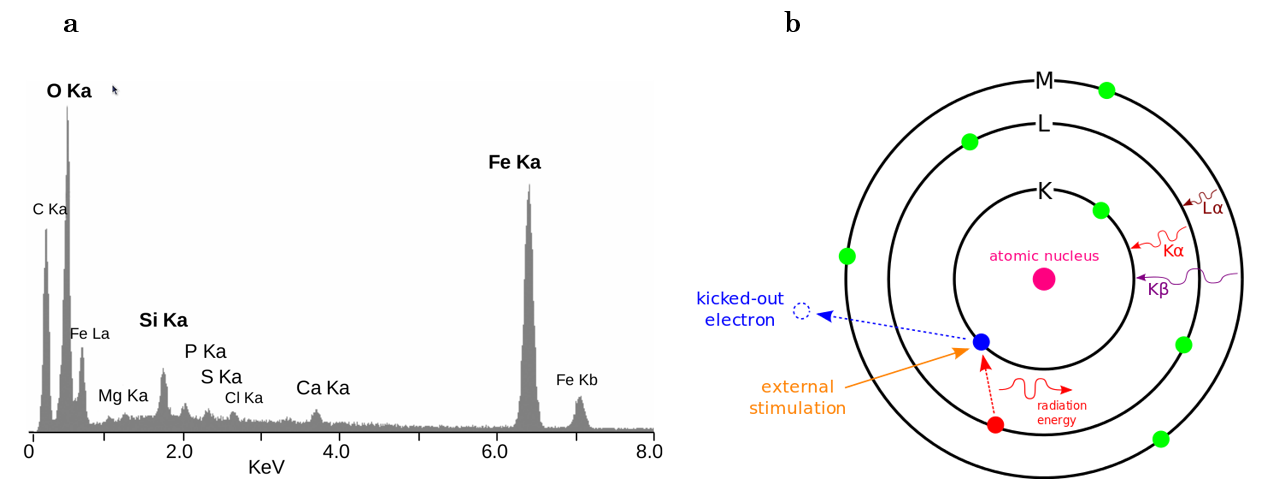
\includegraphics[width=\textwidth]{EDS_set.png}
\caption{(a)EDS频谱示意图\cite{L2008Iron}(b)EDS原理示意图\cite{wiki:eds}}
\label{fig:EDS}
\end{figure}
如图\ref{fig:EDS}所示,电子能谱分析方法的基本思路是利用单色性很好的高频率光源(如激光和X射线)集中照射待分析样品,使得样品表面的原子中的电子被激发到较高价态。 基于量子力学,处于不同量子态的电子其会有不同的动量、角动量乃至自旋的特征的不同分布\cite{Dirac1958The},从而测量这些电子的特征就可以得出材料的特性。\\
\indent 在本文的分析中,对于活性层的纵向切面进行了EDS分析,特别考察了Si元素沿着深度方向的分布情况,有力地佐证了实验测试方法的可行性和实验结果的科学性。